\chapter{Architecture}
\label{chp:architecture} 

This chapter will describe in detail how the different components of the system has been connected together, and how the different protocols has been configured to read and transfer data efficiently. 


\begin{figure}[h]
    \centering
    \includegraphics[scale=0.7]{MasterArchitecture.png}    \caption{System architecture}
    \label{fig:systemArchitecture}
\end{figure}

\newpage

Figure \ref{fig:systemArchitecture} shows how the complete End-to-End system of this thesis is set up. In short terms, the \textit{ADXL345 Accelerometer} is connected to a \textit{Nordic Semiconductor nRF52} using the \gls{i2c} interface. This requires four cables (noted from nRF52 to ADXL345): 

\begin{itemize}
  \item 5V -- VIN 
  \item GND -- GND 
  \item P0.27 -- SDA
  \item P0.26 -- SCL
\end{itemize}


\begin{figure}[h]
    \centering
    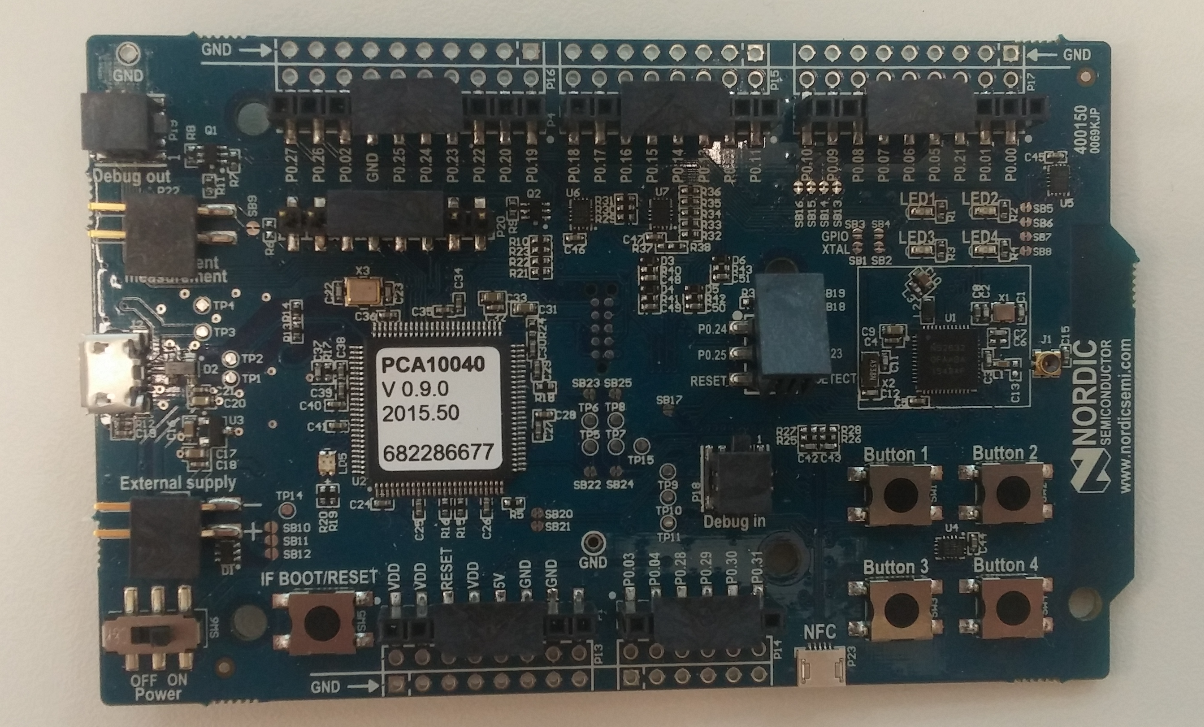
\includegraphics[scale=0.32]{nrf52.png}    \caption{Nordic Semiconductor NRF52}
    \label{fig:adxl345}
\end{figure}

\begin{figure}[h]
    \centering
    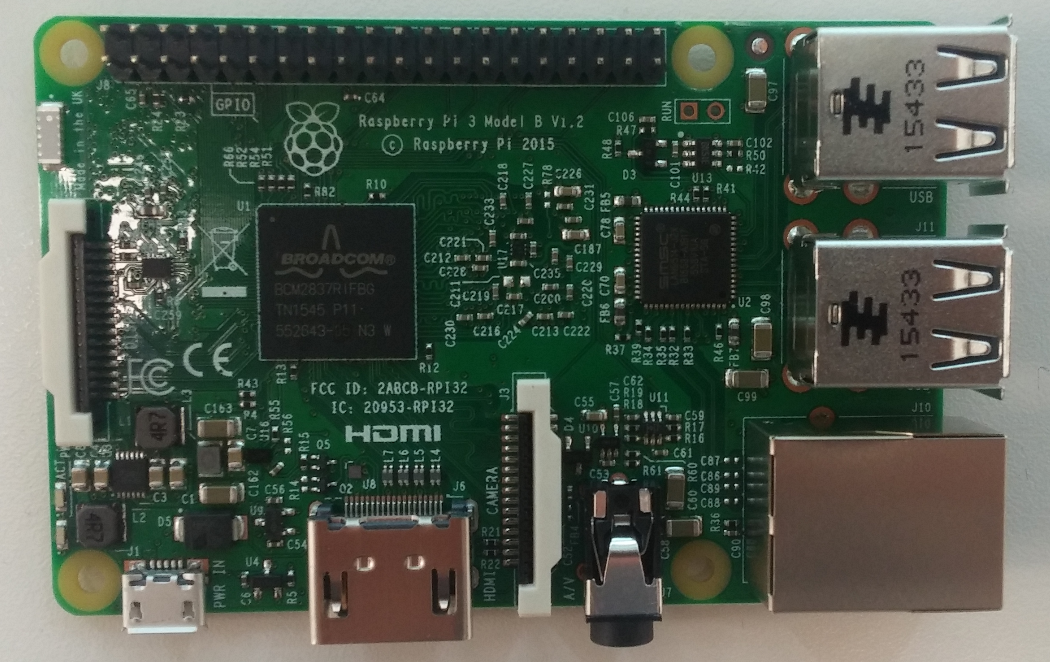
\includegraphics[scale=0.35]{pi3.png}    \caption{Raspberry Pi 3}
    \label{fig:adxl345}
\end{figure}

\begin{figure}[h]
    \centering
    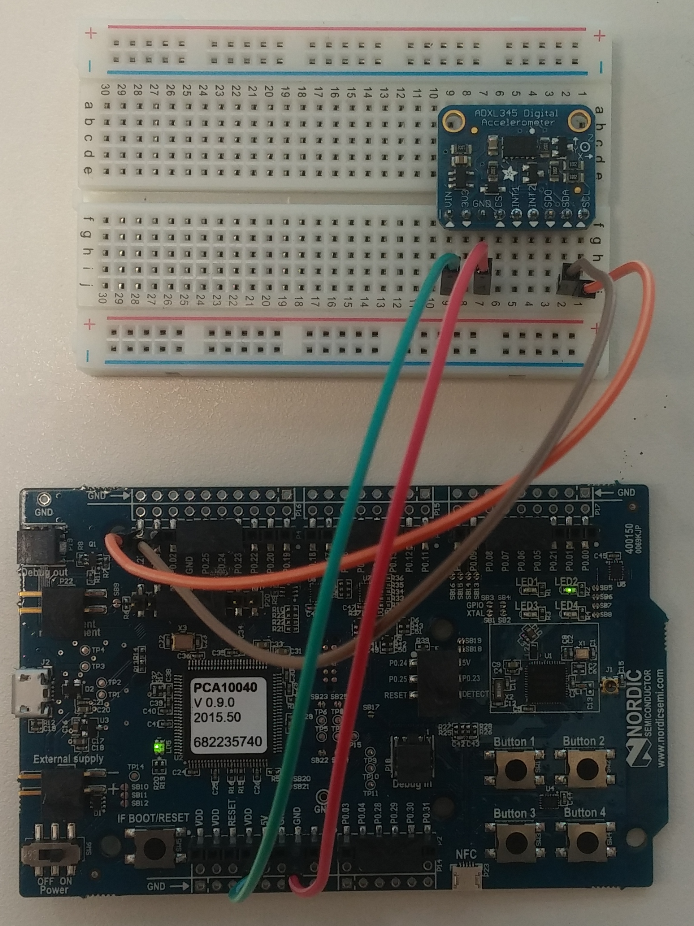
\includegraphics[scale=0.35]{nrf-adxl.png}    \caption{Connected nRF52 -- ADXL345}
    \label{fig:adxl345}
\end{figure}


\section{Enabling \gls{6lowpan} and \gls{ble}}

To enable these things. 

\section{Connecting Raspberry Pi and nRF52}

\section{Connecting nRF52 and ADXL345}

\subsection{\gls{}}

\subsection{\gls{i2c}}


